\subsection{Versuchsaufbau und Durchführung}
\label{abs:Versuchsbaufaufbau_Durchführung}
Die Abbildung \ref{versuchsaufbau} zeigt die Versuchsanordnung. Es handelt sich um einen 4-Punkt-Biegeversuch.   
Dabei wird die Prüfprobe auf zwei Auflagen (rote Dreiecke) positioniert und in den Viertel-Punkten mit der Kraft (\unit[F]) belastet. Die Momentenlinie ist zwischen den Krafteinleitungspunkten konstant und stellt eine Umhüllende, des parabelförmigen Momentenverlaufs, einer äquivalenten Flächenlast dar.

\begin{figure}[h]
\begin{center}
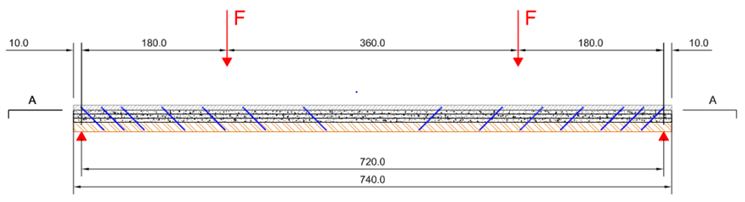
\includegraphics[scale =0.8]{Versuchsaufbau/versuchsaufbau.png}
\caption{Versuchsaufbau mit Lagerung und Lasteinleitung}
\label{versuchsaufbau}
\end{center}
\end{figure}

\subsubsection{Verwendete Messmittel und deren Anordnung}

 Die Wegaufnehmer für die Trägerdurchbiegung wurden in der Trägermitte und unter der Lasteinleitung angeordnet. Weiters wurde auf beiden Trägerenden Wegaufnehmer angebracht, um die Verschiebung zwischen Betonschicht und der BSP-Schicht zu messen. Bei dem ersten und zweiten Großbauteilversuch wurde die Verschiebung noch manuell von den Messuhren abgelesen. Bei den Bauteilversuchen 3 und 4 wurden  digitale Wegaufnehmer verwendet, die anschließend beschrieben werden. 
In der Abbildung \ref{versuchsaufbau} sind die Messpunkte skizziert und beschriftet.

\begin{figure}[h!]
\begin{center}
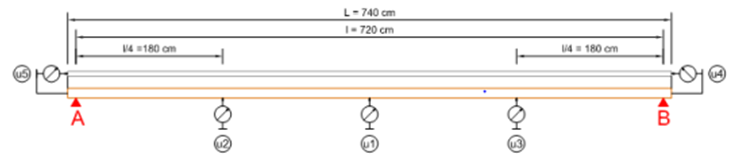
\includegraphics[scale =0.8]{Versuchsaufbau/messanordnung.png}
\caption{Anordnung der Messpunkte beim Bauteilversuch}
\label{versuchsaufbau}
\end{center}
\end{figure}


\begin{figure}[h!]
\begin{center}
	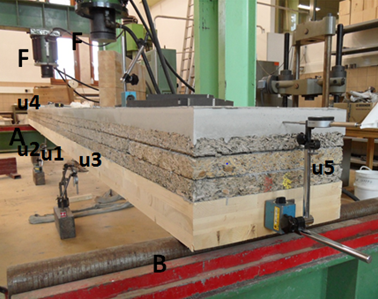
\includegraphics[scale=1.3]{Versuchsaufbau/messpunkte.png}
	\caption{Mess-und Auflagerpunkte beim Bauteilversuch}
	\label{messpunkte}
\end{center}
\end{figure}

	\begin{itemize}
	\item u1.1/ u1.2: Durchbiegung in Feldmitte 	auf beiden Seiten des Trägers
	\item u2/u3: Durchbiegung bei l/4
	\item u4/u5: Verschiebung der Betonschicht 	gegenüber der Holzschicht an beiden 	Enden des Trägers
	\item  Krafteinleitung F bei l/4
	\item A/B: Auflager
	\end{itemize}





\subsubsection{Wegaufnehmer}	

In diesem Abschnitt werden die die verschiedenen Wegaufnehmer beschrieben.

\paragraph{Anologe Wegaufnehmer}

Es wurden analoge Messuhren der Fa. Käfer verwendet. Die Messuhren haben einen Messweg von \unit[7]{cm} und  eine Messgenauigkeit von  \unit[1/100]{mm}.  Auf einen Standfuss wurden die magnetischen Halteeinrichtungen angebracht, welche die Messuhren in der vorgesehenen Position hielten. Der gesamte Aufbau ist in Abbildung \ref{messuhr_unten} dargestellt.

Die Befestigung für die horizontale Verschiebung wurde ebenfalls mit der magnetischen Halteeinrichtung bewerkstelligt. Zuvor musste noch eine Stahlplatte an der BSP-Platte angeschraubt werden, damit die Halteeinrichtung angebracht werden konnte. Der gesamte Aufbau kann Abbildung \ref{messuhr_seitlich} entnommen werden.

\begin{figure}
\begin{minipage}[h]{7cm}
	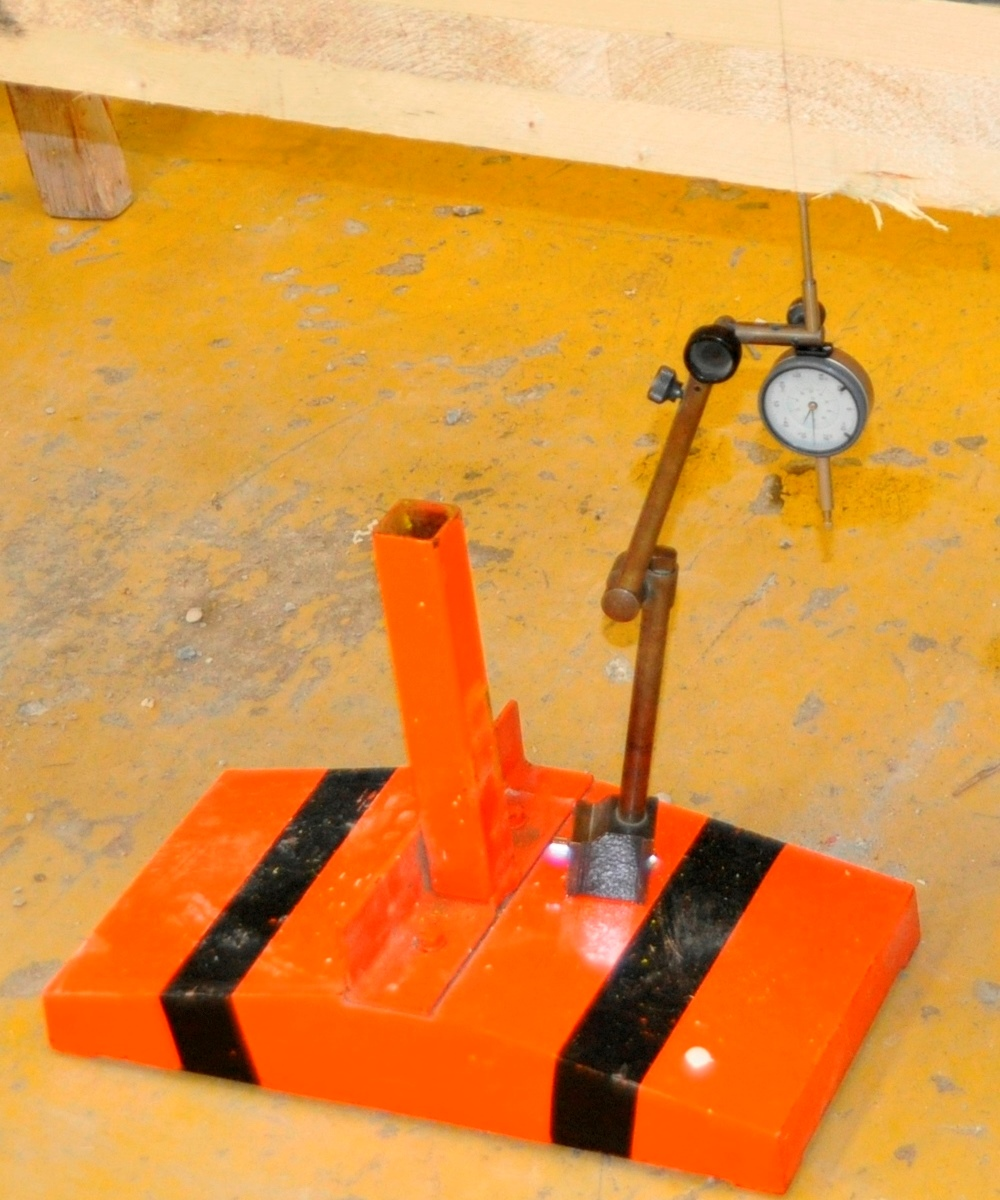
\includegraphics[width=7cm]{Versuchsaufbau/messuhr_unten.jpg}
	\caption{Messuhr für vertikale Verschiebung, befestigt am Standbein}
	\label{messuhr_unten}
\end{minipage}
\hfill
\begin{minipage}[h]{7cm}
	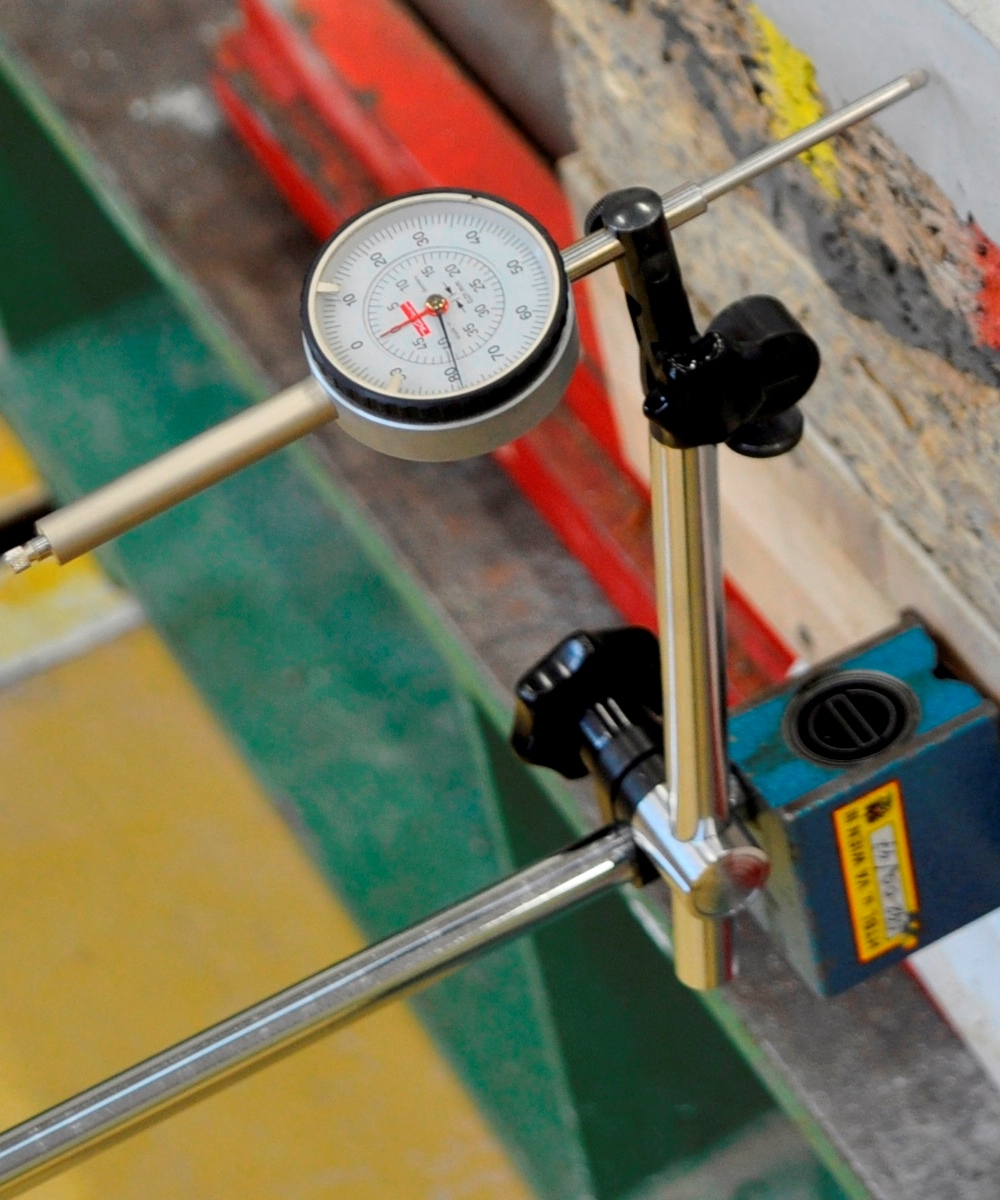
\includegraphics[width=7cm]{Versuchsaufbau/messuhr_seitlich.jpg}
	\caption{Messuhr für horizontale Verschiebung am Bauteilende}
	\label{messuhr_seitlich}
\end{minipage}
\end{figure}


\paragraph{Digitale Wegaufnehmer}

Es wurden digitale Seilzug-Wegsensoren der Fa. MICRO-EPSILON verwendet[Serie WDS, Baureihe P60, \unit[1000]{mm}]. Die Messuhren besaßen einen maximalen Messweg von \unit[100]{cm} und haben eine Messgenauigkeit von \unit[0,24]{mm}. Die Haltevorrichtung für die vertikale Verschiebung, wurde ebenfalls mit dem Standfuss ausgeführt. In den Standfuss wurde eine Metallstange eingeführt und mit kleinen Holzkeilen fixiert. Der  Wegsensor wurde mit M4 Schrauben, Flügelmuttern und einer Holzplatte an der Metallstange montiert. Das Seil wurde mit einer Holzschraube an der BSP-Platte befestigt. Der gesamte Aufbau ist in Abbildung \ref{d_aufnehmer_unten} dargestellt.

Für die Messung der horizontalen Verschiebung, wurde eine Haltevorrichtung herstellt. Die Vorrichung wurde mit Schrauben auf der BSP-Platte angeschraubt. Der Wegsensor wurden ebenfalls mit M4 Schrauben, Flügelmuttern und einer Holzplatte, an der Haltevorrichtung befestigt. Der gesamte Aufbau kann aus  Abbildung \ref{d_aufnehmer_seitlich} entnommen werden.



\begin{figure}[h!]
\begin{minipage}[h!]{7cm}
	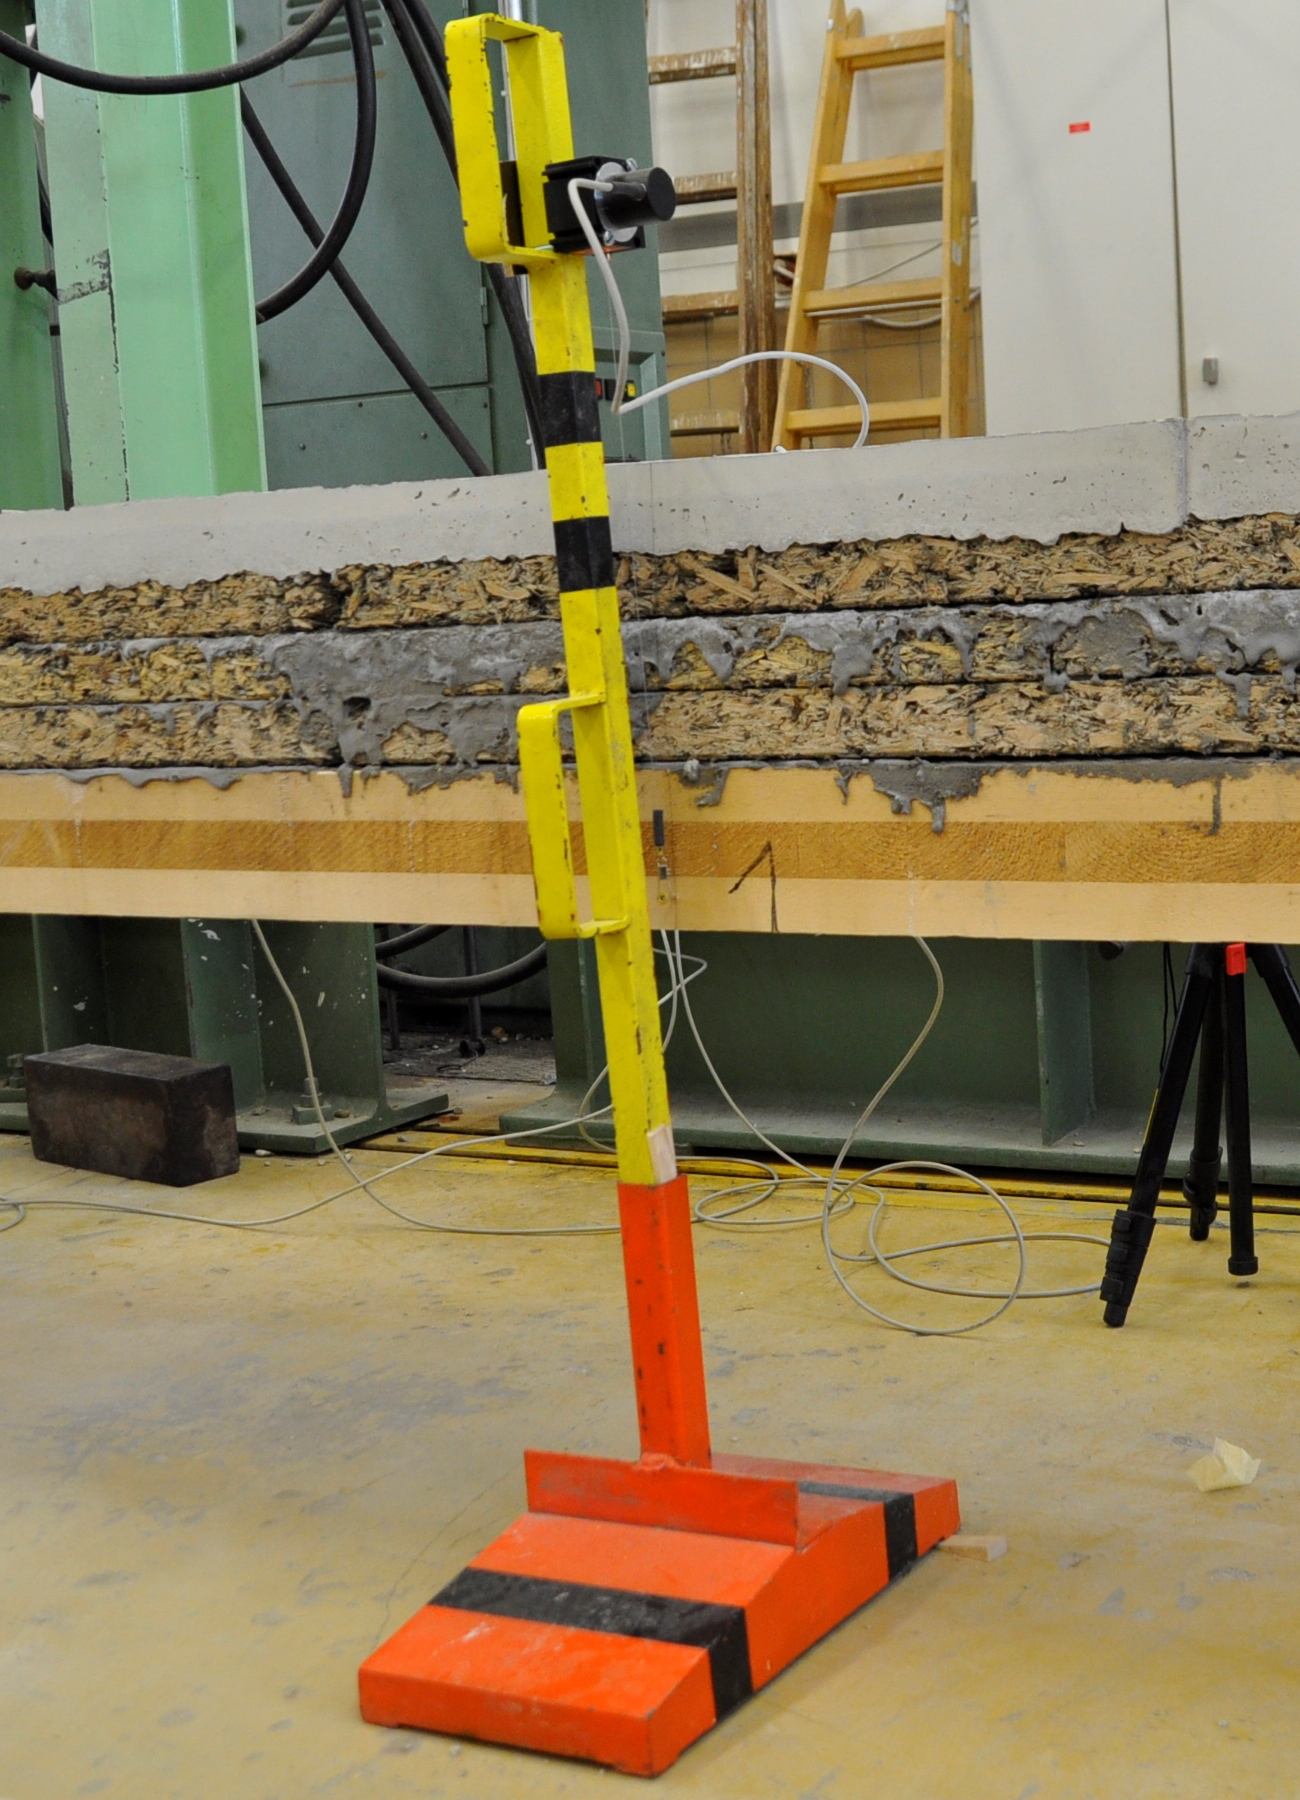
\includegraphics[width=7cm]{Versuchsaufbau/d_aufnehmer_unten.jpg}
	\caption{Wegaufnehmer für vertikale Verschiebung mit Standbein und Stange}
	\label{d_aufnehmer_unten}
\end{minipage}
\hfill
\begin{minipage}[h!]{7cm}
	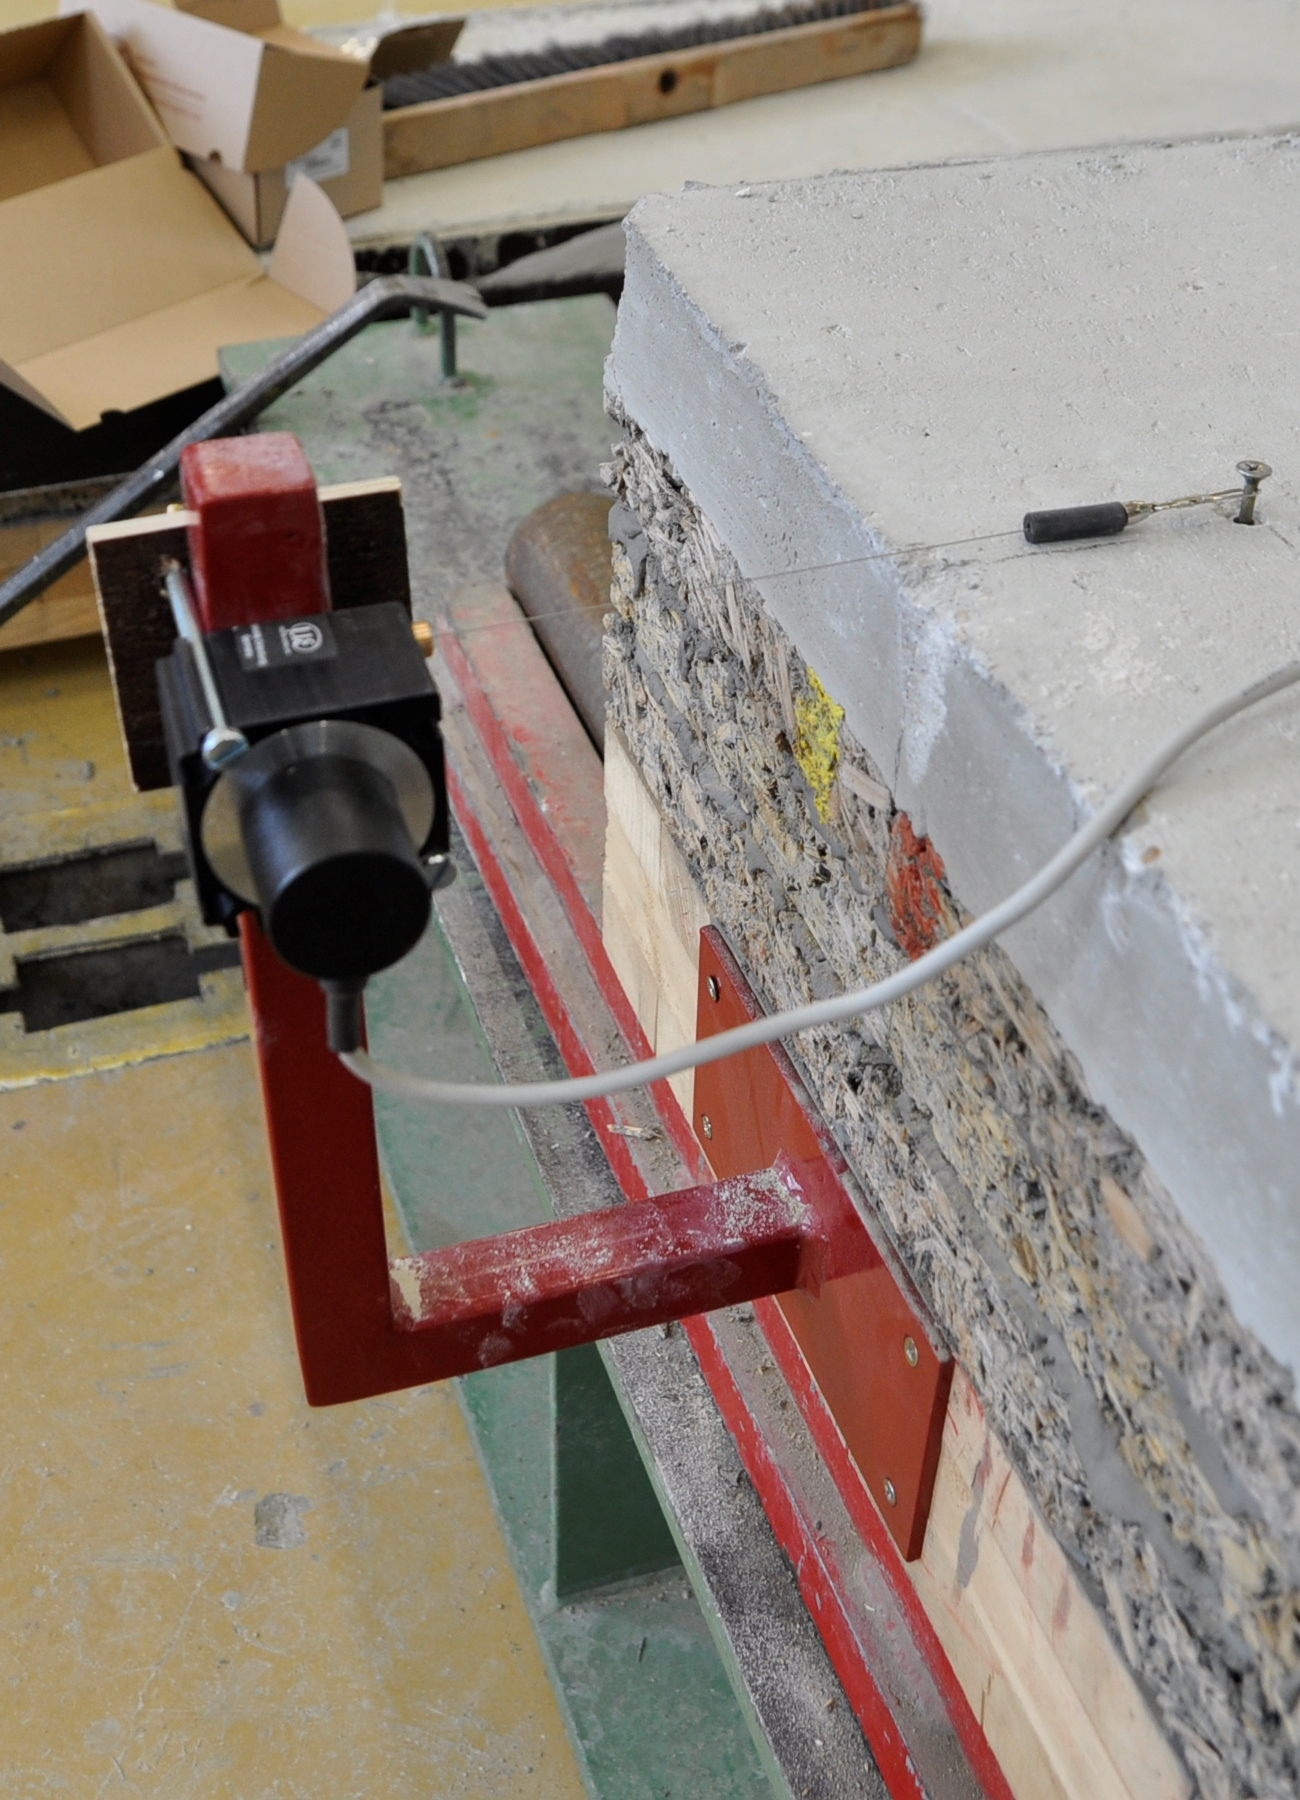
\includegraphics[width=7cm]{Versuchsaufbau/d_aufnehmer_seitlich.jpg}
	\caption{Wegaufnehmer für horizontale Verschiebung am Bauteilende}
	\label{d_aufnehmer_seitlich}
\end{minipage}
\end{figure}










	
\subsubsection{Durchführung des Versuchs}
Der Aufbau des Bauteilversuchs bzw. die Abmessungen des Bauteils ist  Abbildung \ref{versuchsaufbau} zu entnehmen. Für die Bauteilversuche 1 und 2 wurde eine Belastungsgeschwindigkeit von etwa \unit[4]{kN/min} gewählt. Das Ablesen erfolgte in Schritten von \unit[2]{kN}. Bei den Bauteilversuchen 3 und 4 wurde eine vorgegebene Belastungskurve gewählt. Die Kurve wurde der Norm [ÖN EN 380] entnommen. Das Grundverfahren der Belastung besteht aus den 7 Verfahrensstufen. 

\paragraph{Belastungserklärung}
\begin{itemize}
\item $G_{1}$\ldots Eigengewicht des Bauteils
\item $G_{2}$\ldots Gewicht des erforderlichen Aufbaus (Dämmung, Estrich, Bodenbelag)
\item $Q$ \ldots veränderliche Last lt. EC1 für Wohnräume
\item Belastungsgeschwindigkeit: \unit[1,5]{kN/min}
\item Die Lastangaben beziehen sich auf einen Zylinder.
\end{itemize}
	

\begin{figure}
\begin{center}

	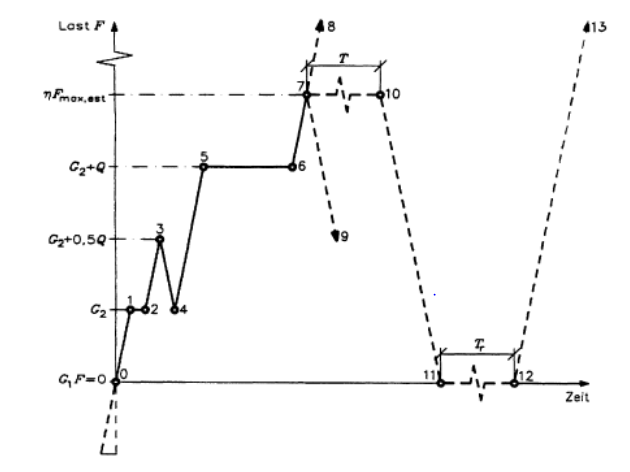
\includegraphics[width=12cm]{Versuchsaufbau/belastungskurve.png}
	\caption{Schematische Belasungskurve, nach []}
	\label{belastungskurve}

\end{center}	
\end{figure}	

\begin{table}
\caption{Grundlagen der Belastung,[]}
\begin{center}
\begin{tabular}{|c|c|c|c|}
\hline 
Verfahrensstufe & Belastungsverfahren & Zeit in [s] & F [kN] \\ 
\hline \hline
0 & Es wirkt nur G;F=0 &  &  \\ 
\hline 
0-1 & F=G aufbringen &  & 2,70 \\ 
\hline 
1-2 & F=G konstant halten & 120 & 2,70 \\ 
\hline 
2-3 & F=G+0,5*Q aufbringen & 120 & 5,40 \\ 
\hline 
3-4 & 0,5 Q entlasten & 120 & 2,70 \\ 
\hline 
4-5 & F=G+Q aufbringen & 240 & 8,10 \\ 
\hline 
5-6 & F=G+Q konstant halten & 600 & 8,10 \\ 
\hline 
6-8 & F= steigern bis Bruch &  &  \\ 
\hline \hline
\multicolumn{4}{|c|}{ max. Belastungsgeschwindigkeit 0,25Q je 60 sec} \\ 
\hline 
\end{tabular} 
\label{tab:belastung}
\end{center}
\end{table}